\chapter{Resultados Obtidos} \label{capitulo4}

O objetivo deste capítulo é apresentar os resultados obtidos a partir da metodologia desenvolvida no capítulo \ref{metodologia}. É realizado um exercício prático que visa melhor entender as expressões que as reniões do banco central desejam transmitir por meio das atas. Utilizaremos, entretanto, suas versões em inglês (\textit{minutes}), devido ao fato de não haver dicionários léxicos em português que permita um tratamento às atas.

O trabalho feito aqui é referente ao período de 2003-2018. Que por sua vez compete da gestão Meirelles à gestão Ian Goldfajn frente ao BCB -- do governo Lula ao governo Temer. Vale salientar, além disto, o \textit{software}/linguagem de programação utilizado: este trabalho foi feito exclusivamente por meio da linguagem R \cite{cran}. Sua escolha foi devido a esta linguagem ser considerada moderna e de alto nível, possibilitando de forma simples uma análise robusta dos dados. Ainda, por ser uma linguagem de programação voltada para estatística, como no próprio manual ``feita por estatísticos, para estatísticos'', o R possibilita uma vasta gama de opções para análise textual e de dados. Os códigos deste capítulo, bem como deste trabalho estão disponíveis no \href{https://github.com/gustavovital/Monografia}{repositório online da monografia} \url{https://github.com/gustavovital/Monografia}.

\section{Base de dados}

De acordo com o período analisado, de 2003 à 2018, foram disponibilizadas 140 atas do BCB das respectivas reuniões. Dessa forma, totaliza-se 140 reuniões do COPOM. A partir de um algoritmo de \textit{web scraping}, acessamos essas atas e fizemos download, das suas correspondentes em inglês (\textit{minutes}).

O período escolhido é relacionado com as mudanças políticas e econômicas no Brasil, levando em consideração, também, o tamanho amostral, afim de compreendermos melhor o que se passou nesses anos.

%\subsection{Obtenção da Base de Dados}

%Como dito anteriormente, foi utilizado um algoritmo de \textit{web scraping} para a obtenção das atas do COPOM. 

Inicialmente, por meio do pacote \textit{rvest} \cite{rvest} descobrimos as URL's referentes as atas do COPOM - isso é, de todas. Feito isto, obtemos as URL's por meio do pacote ``\textbf{cronoAno a}''\footnote{http://selectorgadget.com/}, bem como obtemos os links das atas.

Por meio de uma estrutura de repetição simples armazenamos estas atas em listas e realizamos os \textit{downloads} das atas, já do período selecionado, 2003-2018 . Armazenamos estas num diretório.

Utilizando o pacote \textit{tm} \cite{tm}, fazemos a leitura dos PDF's e criamos um \textit{dataframe} que contém os \textit{corpus}\footnote{Efetivamente os textos que iremos trabalhar neste \textit{corpus}, contém basicamente os caracteres das leituras dos PDF's} das atas. Nosso \textit{dataframe} fica com três colunas (numero da ata, nome do PDF, e \textit{corpus}) e 140 linhas (cada uma referente a uma ata). 

Para cada \textit{corpus} contido no documento aplicamos uma técnica de \textit{stop words}, por meio do dicionário \textit{stopwords} \cite{tidystop}, e adicionamos palavras que julgamos ser desnecessárias, assumindo que tal palavra aparece \textit{pelo menos} 400 vezes no total dos corpus. Dentre as palavras que desconsideramos, podemos citar como exemplo numerais ou nomes próprios sem relevância para uma análise econômica. Além disso, removemos palavras com erro de leitura devido a quebra de linhas (por exemplo \texttt{ninflation})\footnote{As palavras com erro de leitura foram desconsideradas nesta parte do processo. Na contagem geral de palavras, passamos a considerar, por essas poderem interferir no resultado final.}.
\begin{figure}[!h]
    \centering
    \caption{Núvem de palavras das palavras que mais aparecem nas atas do COPOM durante todo o período analisado}
    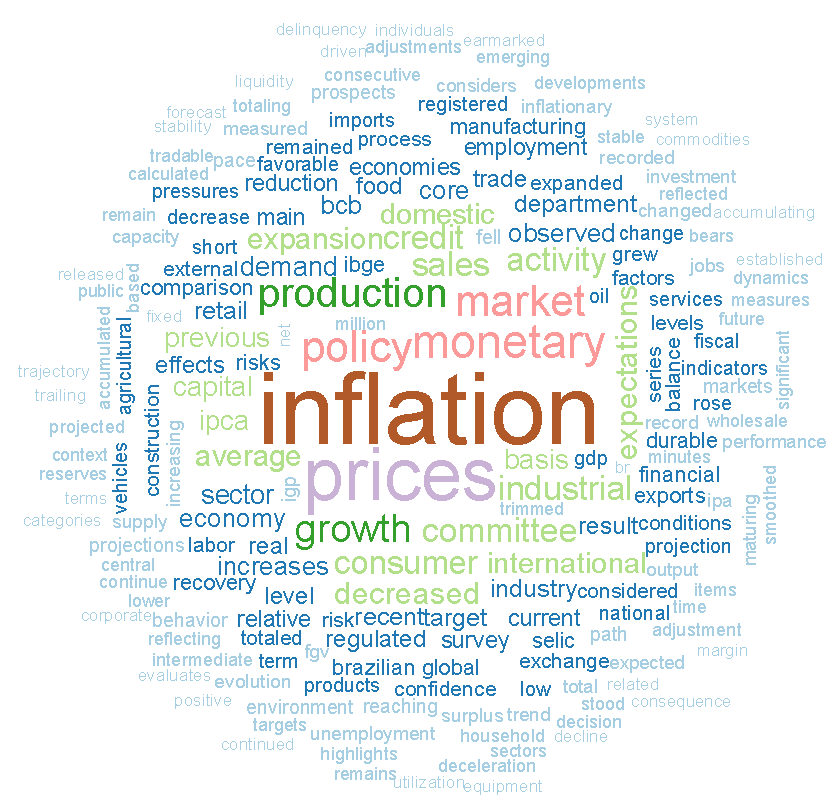
\includegraphics[width=.8\textwidth]{capitulos/figures/wordcloud.pdf}
    \fonte{BCB. Elaboração própria}
    \label{fig:wc01}
\end{figure}

A Figura \ref{fig:wc01} apresenta em escala as palavras que mais aparecem nas atas do COPOM, levando em consideração a técnica aplicada de \textit{stopwords}. Nitidamente, nos atentamos ao fato de \textbf{inflation}, \textbf{prices}, e \textbf{market} tomarem o primeiro plano, quanto a nossa atenção às palavras mais recorrentes.

\subsection{Estatísticas Descritivas}

O primeiro \textit{dataframe} de análise que obtemos diz respeito as frequências das palavras de cunho econômico. Feito isso, é interessante uma contagem das palavras. Na Tabela \ref{tab:contgeral}, podemos ver as palavras que mais aparecem nas atas do COPOM no período estudado. Ainda, devemos salientar:  essa é a contagem ``\textbf{líquida}'' das palavras - isso é, já foi feita a correção relativa às palavras repetidas ou não contabilizadas\footnote{Por exemplo, na contagem bruta, teríamos levado em consideração palavras como \textit{nprices, price} e \textit{nprices}}. 

\begin{table}[!h]
\centering
\caption{Palavras que mais aparecem nas atas do COPOM (2003-2018)}
\begin{tabular}{ll|ll|ll|ll}
\hline
Palavra    & n    & Palavra      & n    & Palavra       & n    & Palavra   & n    \\ \hline
inflation  & 7370 & committee    & 1785 & decreased     & 1579 & capital   & 1279 \\
prices     & 5079 & industrial   & 1785 & expansion     & 1468 & ipca      & 1256 \\
monetary   & 2882 & sales        & 1778 & average       & 1433 & demand    & 1221 \\
policy     & 2651 & credit       & 1775 & international & 1427 & sector    & 1187 \\
market     & 2562 & consumer     & 1701 & domestic      & 1364 & economy   & 1166 \\
production & 2373 & activity     & 1698 & previous      & 1327 & observed  & 1159 \\
growth     & 2194 & expectations & 1593 & basis         & 1316 & increases & 1157 \\ \hline
\end{tabular}
\label{tab:contgeral}
\end{table}

Dito isso, pode-se, também, apresentar a contagem das palavras referente aos períodos específicos analisados. As Tabelas \ref{tab:contmeir}, \ref{tab:conttom}, e \ref{tab:contian} apresentam essas contagens.

\begin{table}[h]
\centering
\caption{Palavras que mais aparecem nas atas do COPOM (período Meirelles)}
\begin{tabular}{llllllll}
  \hline
Palavra & n & Palavra & n & Palavra & n & Palavra & n \\ 
  \hline
inflation & 4348 & industrial & 1329 & consumer & 1033 & activity & 926 \\ 
prices & 3212 & growth & 1272 & expansion & 983 & domestic & 926 \\ 
market & 1595 & policy & 1259 & average & 977 & expectations & 907 \\ 
production & 1559 & sales & 1211 & ipca & 935 & previous & 871 \\ 
monetary & 1395 & credit & 1162 & basis & 932 & capital & 864 \\ 
   \hline
\end{tabular}
\label{tab:contmeir}
\end{table}

\begin{table}[h]
\centering
\caption{Palavras que mais aparecem nas atas do COPOM (período Tombini)}
\begin{tabular}{llllllll}
  \hline
Palavra & n & Palavra & n & Palavra & n & Palavra & n \\ 
  \hline
inflation & 2377 & growth & 903 & activity & 607 & sector & 500 \\ 
  prices & 1781 & committee & 844 & credit & 605 & bcb & 492 \\ 
  monetary & 995 & production & 813 & sales & 567 & expansion & 477 \\ 
  policy & 960 & decreased & 754 & industry & 564 & observed & 475 \\ 
  market & 919 & consumer & 663 & international & 526 & changed & 473 \\ 
   \hline
\end{tabular}
\label{tab:conttom}
\end{table}

\begin{table}[!h]
\centering
\caption{Palavras que mais aparecem nas atas do COPOM (período Goldfajn)}
\begin{tabular}{llllllll}
  \hline
Palavra & n & Palavra & n & Palavra & n & Palavra & n \\ 
  \hline
inflation & 645 & expectations & 246 & brazilian & 156 & easing & 117 \\ 
  monetary & 492 & risks & 211 & baseline & 153 & projections & 117 \\ 
  policy & 432 & activity & 165 & balance & 126 & governor & 116 \\ 
  committee & 429 & department & 165 & central & 119 & process & 116 \\ 
  economy & 306 & evolution & 165 & adjustments & 118 & risk & 116 \\ 
   \hline
\end{tabular}
\label{tab:contian}
\end{table}

Trivialmente, percebemos que a palavra que mais aparece nas atas é \textit{inflation}. O controle da inflação frente a meta para a inflação é um dos pontos de interesse do BC, além disso temos que levar em consideração o crescimento da inflação ao final do governo Dilma. \textit{Price} deixa de aparecer como uma palavra importante nas atas da gestão Goldfajn e \textit{policy} não aparece nas atas referentes ao governo Lula.

A partir da contagem total das palavras\footnote{O \textit{dataframe} referente possui mais de 12.000 palavras identificadas, dentre as quais considera-se numeral como um caractere} devemos definir nosso objeto de estudo. Trabalharemos com as 10 palavras de cunho econômico que mais aparecem nas atas do COPOM.

Alguns pontos têm que ser considerados. Primeiramente, esse estudo prevê um período de 16 anos, um total de 140 atas. Entretanto, os períodos de gestão do BCB não foram regulares, e mesmo que fossem, não poderíamos supor que o número de atas por período seria o mesmo, bem como os tamanhos das atas.

\subsection{Frequência das Principais Palavras}

Das 140 atas que utilizamos, no período Lula (gestão Meirelles) temos um total de 76 atas; no período Dilma (gestão Tombini) temos um total de 45 atas; por fim, no período Temer (gestão Goldfajn) temos um total de 19 atas. Ainda, a partir das 10 palavras \textit{de cunho econômico} que mais aparecem nas atas do COPOM, podemos fazer um estudo dirigido para cada período. Inicialmente, vamos considerar os valores \textit{absolutos} das palavras - isso é, a simples contagem de quantas vezes cada palavra aparece, independentemente do tamanho da ata\footnote{Ver repositório online}. 

As palavras que mais aparecem em cada período, como já exposto anteriormente, se encontram nas Tabelas \ref{tab:contmeir}, \ref{tab:conttom}, e \ref{tab:contian}. Podemos, agora, ilustrar, por meio de um histograma, suas distribuições; e um gráfico de linha, para em relação às ocorrências das palavras.

Inicialmente, como feito na seção anterior, faremos isso para todos os períodos (2003-2018)\footnote{Ver repositório online}. A distribuição das palavras acaba por não seguir um distribuição identificável visualmente. Nos histogramas, podemos notar isso quando em relação aos \textit{kernels} apresentados. As figuras estão disponíveis no repositório da Monografia.

\subsection{Frequências Relativas}

Como é possível perceber, se fossemos trabalhar com as ocorrências das palavras de forma \textit{absoluta}, teríamos um problema notável: como os tamanhos das atas variam, não poderíamos comparar as ocorrências das palavras de forma direta. Desta forma, como metodologia utilizada, passaremos a considerar as frequências relativas das palavras em relação a cada ata.

Basicamente, a metodologia utilizada foi, dado o número de ocorrências de uma palavra, divide-se este número pelo total de palavras nas atas - já desconsiderado as palavras de dicionários de \textit{stopwords}, tal que:
$$Fp_i = \frac{p_i}{N_i}$$
\noindent
em que $Fp_i$ é a frequência da palavra $p$, dada por $\frac{p_i}{N_i}$; ou seja, o número de ocorrências da palavra $p$, dividido pelo número total de ocorrência de todas as palavras $N$, na ata $i$.

Podemos perceber um tendência principal nas palavras \textit{inflation} e \textit{monetary}, possivelmente relacionada com a conjuntura econômica que o país vivia - crise econômica acentuada em 2015. Enquanto, por exemplo, \textit{prices}, \textit{industrial}, \textit{credit}, \textit{growth}, \textit{consumer}, e \textit{market} praticamente deixam de aparecer no período Goldfajn - por vezes nem aparecem, se referem somente ao responsável da sessão, no BC, isso é não há nenhuma interpretação econômica para essas palavras nas atas no período pós-impeachment

É possível ainda, sugerir uma interpretação econômica para o desaparecimento dessas palavras. Se analisarmos o caso das palavras \textit{monetary} e \textit{policy}, percebemos que a correlação das frequências dessas palavras é de \texttt{0.973746}, nos dando um indício de que essas são utilizadas conjuntamente, em \textit{monetary policy} - de tal forma que isso indique que o andamento dessas palavras se refira ao tratamento com a política monetária\footnote{Não utilizamos essa técnica de trabalho neste documento. Se fosse o objetivo trabalhar com conjuntos de palavras, trabalharíamos com \textit{clusters}}.  

\begin{figure}[!h]
    \centering
    \caption{Comparação das frequências de \textit{Monetary} e \textit{Policy}}
    \includegraphics[width=\textwidth]{capitulos/figures/policy_monetary_ggplot.pdf}
    \fonte{BCB. Elaboração própria}
    \label{fig:monetarypolicy}
\end{figure}

A Figura \ref{fig:monetarypolicy} apresenta as frequências relativas às atas das palavras \textit{monetary} e \textit{policy} no decorrer do período analisado. Nitidamente, é possível verificar uma correlação dessas duas palavras. 

\begin{figure}[!h]
    \centering
    \caption{Comparação das frequências de \textit{Monetary} e \textit{Policy} com o IPCA acumulado em 12 meses}
    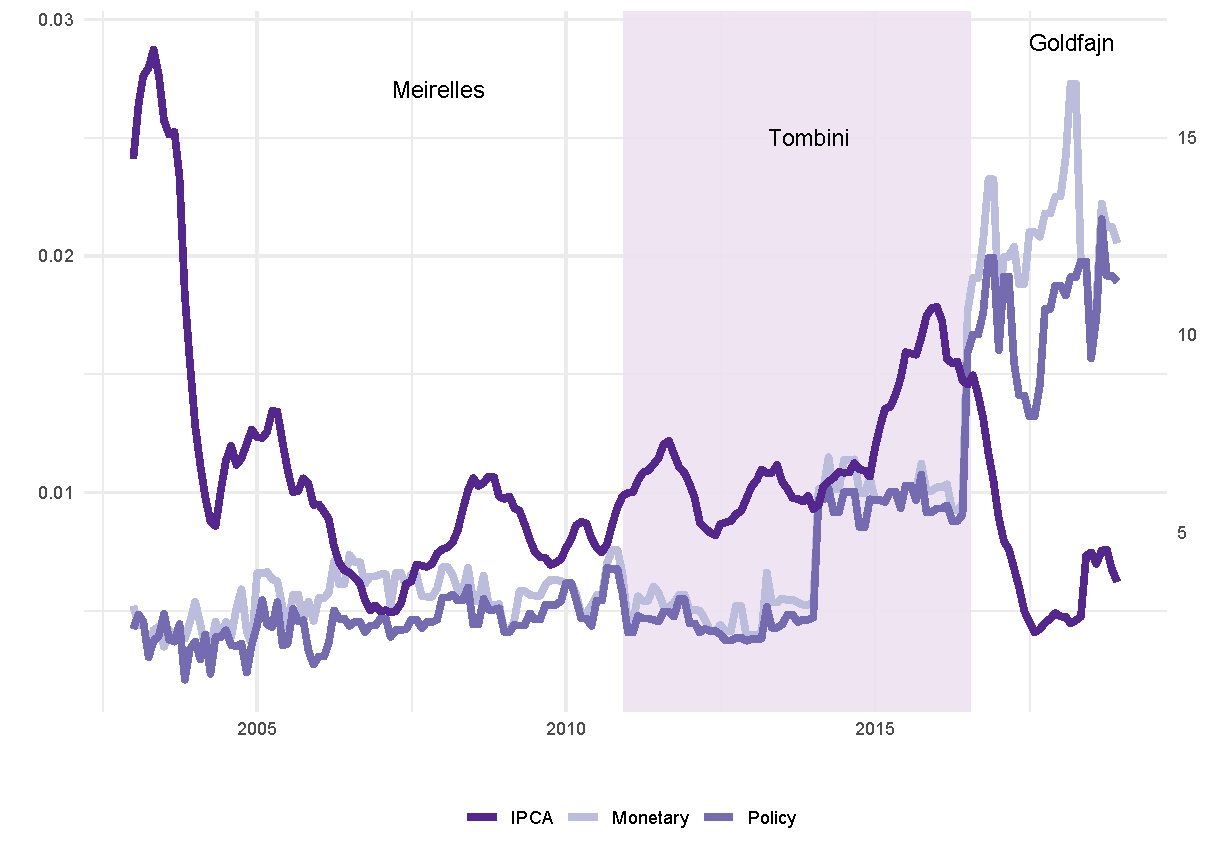
\includegraphics[width=\textwidth]{capitulos/figures/graficoipcapolicy.pdf}
    \fonte{BCB. Elaboração própria}
    \label{fig:monpolipca}
\end{figure}

A Figura \ref{fig:monpolipca} apresenta a evolução do ipca acumulado em 12 meses de acordo com os períodos de gestão do BCB, isso é: o aumento em relação a frequência do aparecimento das palavras \textit{policy} e \textit{monetary} pode estar relacionado com uma possível ênfase a mudança de política monetária adotada pelo BC. A partir de 2015 há um \textit{boom} na inflação acumulada, sendo o tratamento dessa uma prioridade, faz sentido que se espere uma mudança em relação à política monetária, se esta não estiver surtindo efeito.

\section{A divergência de Kullback-Liebler nas frequências das Atas do COPOM}

Como primeiro exercício prático deste trabalho, é proposto o cálculo da divergência de K-L. Isso é, verificaremos se as expressões das atas nos períodos analisados possuem similaridades com base nas 148 palavras que mais aparecem no conjunto dos 140 \textit{minutes} do COPOM. Num primeiro momento, a intenção foi o cálculo das 200 palavras que mais aparecem nas atas, entretanto, durante o período Goldfajn algumas palavras deixam de aparecer\footnote{As palavras que deixam de aparecer nas atas são: sales, basis, capital, industry, comparison, ibge, exports, durable, manufacturing, expanded, grew, series, construction, totaled, rose, oil, registered, agricultural, imports, products, vehicles, igp, surplus, jobs, recorded, record, output, ipa, fgv, maturing, intermediate, household, smoothed, totaling, calculated, bears, million, trimmed, tradable, liquidity, driven, trailing, br, categories, evaluates, earmarked, equipment, individuals, net, delinquency, commodities, fixed}, já como um indício de mudança em relação a abordagem de política monetária e -- assim -- não seria possível o cálculo da divergência de K-L. 

Como o tamanho das atas variam de período a período analisado -- bem como de ata para ata -- foi necessário trabalharmos com a frequência relativa dessas palavras.

%A diferença de K-L é uma medida, dentro do campo da teoria da informação, capaz de mensurar o quanto uma distribuição $f(x)$ é \textit{próxima} a uma distribuição $g(x0)$. Como apresentado no capítulo \ref{metodologia}, para o caso discreto, esta é calculada da seguinte forma:
%\begin{align*}
%I(f, g) = \sum_{i=1}^{k} p(x_{i}) \cdot \log\left( \frac{p(x_{i})}{q(x_{i})}\right)
%\end{align*}
%\noindent
%a fim de aplicarmos essa medida de distância, podemos considerar a equação da seguinte forma: 1 - considerando $f(x)$ a distribuição para as atas do período Meirelles e $g(x)$ para o período Goldfajn, teríamos que a divergência de K-L seria dada como o somatório das distribuições das palavras do período Meirelles multiplicado pelo logaritmo natural da diferença das distribuições de palavras do período Meirelles pela distribuições de palavras do período Goldfajn.

É sabido que a política monetária adotada pelos períodos Meirelles e Tombini foram políticas monetárias sobre vigência do \textit{Partido dos Trabalhadores} (PT); por um outro lado, durante o período Goldfajn, o partido vigente foi o Partido do Movimento Democrático Brasileiro (PMDB). É esperado então que haja uma similaridade maior em relação aos períodos Meirelles-Tombini do que, por exemplo, os períodos Meirelles-Goldfajn. Ainda, podemos assumir uma possível transição de política monetária no que diz respeito ao período Tombini -- dessa forma, consideramos as distribuições de palavras, ou expressão das atas, levando em consideração três períodos distintos de política brasileira: Meirelles (Lula), Tombini (Dilma), e Goldfajn (Temer).

\subsection{Análise para os Períodos de Gestão do Banco Central}

Essa subseção é dividida em três partes. Na primeira faremos uma análise levando em consideração como distribuição das palavras tomando como referência o período Meirelles, na segunda o período Tombini, e por fim o período Goldfajn. Isso é necessário pois a medida de informação de K-L não é uma medida simétrica, logo quando analisada tomando como referência o período Meirelles contra, por exemplo o período Tombini, não teríamos o mesmo resultado quando tomando o período Tombini como referência. Ao final é apresentado uma tabela geral com os valores da divergência de K-L para as 10, 20, 50, 100, e 148 palavras.

\subsubsection*{Período Meirelles}

A primeira comparação feita é em relação ao período Meirelles. Tomando a distribuição de palavras desse período como referência, é calculado o valor da divergência de K-L em comparação aos outros dois períodos: Tombini e Goldfajn.

\begin{figure}[!h]
    \centering
    \caption{Divergência de K-L conforme o acréscimo de palavras para o cálculo (período Meirelles)}
    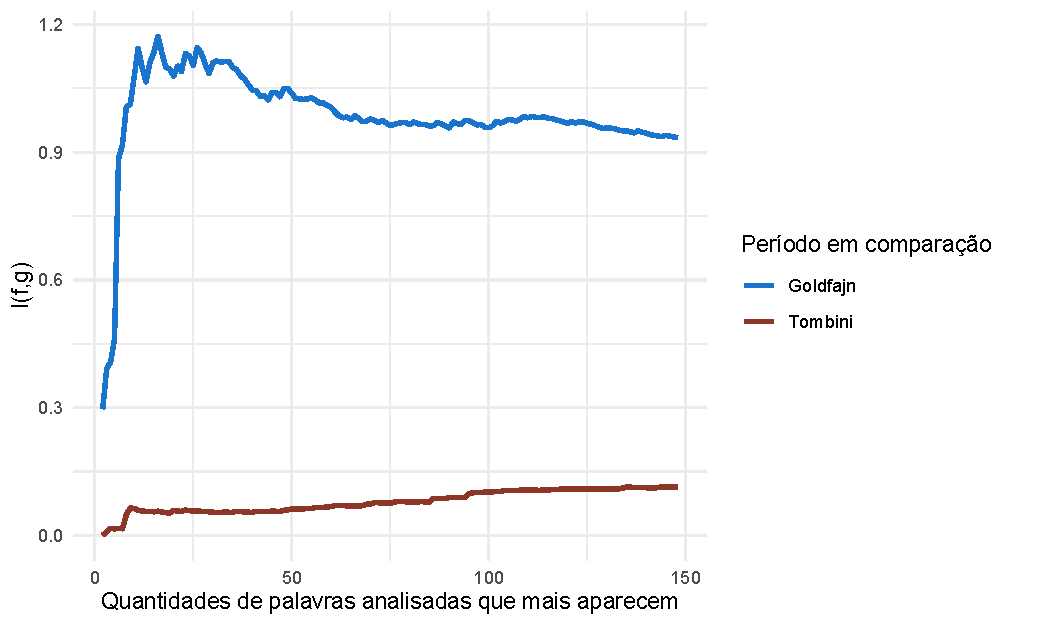
\includegraphics[width=\textwidth]{capitulos/figures/klmeirelles.pdf}
    \fonte{Elaboração própria.}
    \label{fig:klmeirelles}
\end{figure}

A Figura \ref{fig:klmeirelles} apresenta a evolução da divergência de K-L conforme o acréscimo das palavras que mais aparecem nas atas. Nitidamente, as distribuições de palavras do período Meirelles se aproxima da distribuições de palavras do período Tombini de forma mais expressiva do que do período Goldfajn, com uma diferença mínima próxima a 0.3 no valor do critério de K-L.

\subsubsection*{Período Tombini}

Tomando a distribuição de palavras do período Tombini como referência, é calculado o valor da divergência de K-L em comparação aos outros dois períodos: Meirelles e Goldfajn.

\begin{figure}[!h]
    \centering
    \caption{Divergência de K-L conforme o acréscimo de palavras para o cálculo (período Tombini)}
    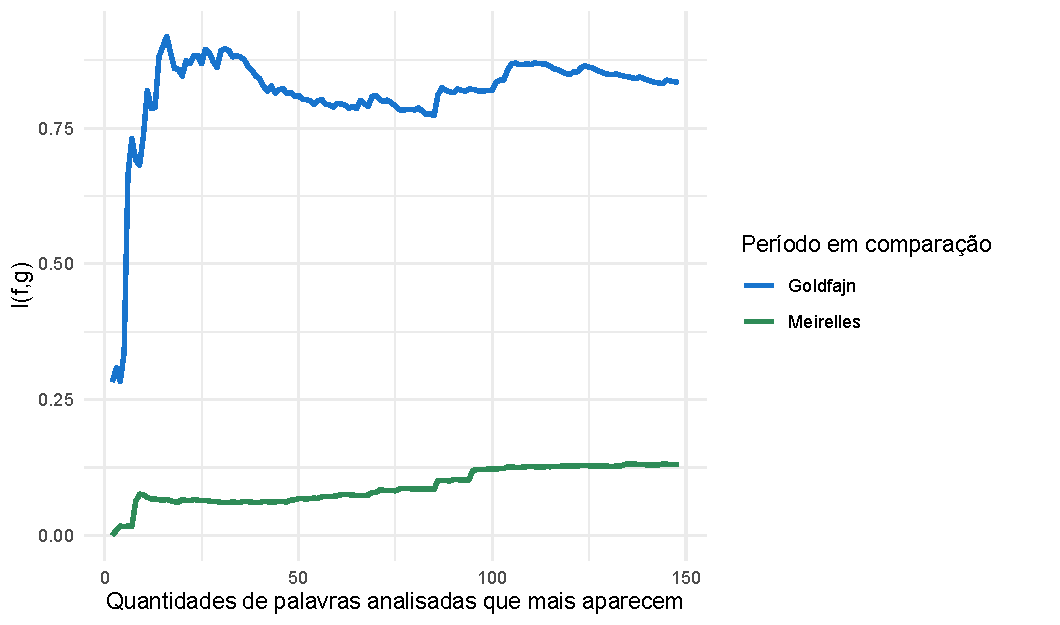
\includegraphics[width=\textwidth]{capitulos/figures/kltombini.pdf}
    \fonte{Elaboração própria.}
    \label{fig:kltombini}
\end{figure}

A Figura \ref{fig:kltombini} apresenta, então, a evolução da divergência de K-L conforme o acréscimo das palavras que mais aparecem nas atas quando tomamos por referência o período Tombini. Nitidamente, as distribuições de palavras desse período analisado se aproxima da distribuições de palavras do período Meirelles de forma mais expressiva -- novamente -- do que do período Goldfajn, com uma diferença mínima próxima a 0.25 no valor do critério de K-L.

É enfatizado, então, uma semelhança quando as distribuições de palavras estão contidas num período de mesma gestão política vigente (PT); enquanto quando comparado ao período político PMDB as distribuições se tornam mais distantes.

\subsubsection*{Período Goldfajn}

Por fim, analisa-se como período de referência a gestão Goldfajn. Então, é feita uma comparação frente aos outros dois períodos: período Meirelles e período Tombini.

Como já apresentado, é esperado que essa distribuição de palavras seja mais distinta à distribuição de palavras da gestão Meirelles -- consequentemente mais próxima a gestão Tombini.

\begin{figure}[!h]
    \centering
    \caption{Divergência de K-L conforme o acréscimo de palavras para o cálculo (período Tombini)}
    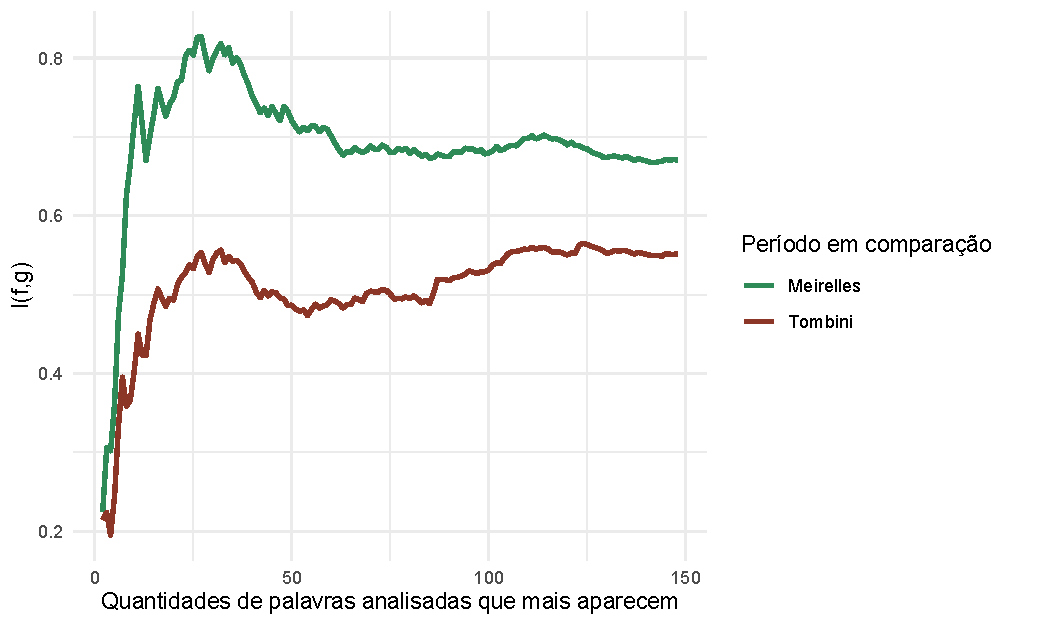
\includegraphics[width=\textwidth]{capitulos/figures/klgoldfajn.pdf}
    \fonte{Elaboração própria.}
    \label{fig:klgoldfajn}
\end{figure}

De fato, a Figura \ref{fig:klgoldfajn} demonstra que ainda que as distâncias das distribuições tenham sido reduzidas (quando o período Goldfajn é referência), elas ainda indicam uma proximidade maior ao período Tombini do que ao período Meirelles.

De forma geral, podemos apresentar os resultados das Figuras \ref{fig:klmeirelles}, \ref{fig:kltombini} e \ref{fig:klgoldfajn} como um indicador do que acontece frente as expressões das atas no que diz repeito ao âmbito de política monetária. Isso é, no período Meirelles a distribuição de palavras realmente se assemelha mais ao período Tombini e menos ao período Goldfajn. Seja pela própria política monetária ou mesmo em relação ao âmbito de um outro cenário macroeconômico.

Uma outra abordagem que pode ser levada em consideração é em relação aos termos econômicos. Conforme o número de palavras nas distribuições aumentam a tendência é que menos palavras sejam relacionadas a questão econômica/conjuntural vigente em um determinado período.

Se nos atentarmos as dez palavras mais recorrentes, teremos -- em ordem: \textit{inflation, prices, market, production, monetary, industrial, growth, policy, sales,} e \textit{credit}. Entretanto, e obviamente, de \textbf{todas} as palavras analisadas, nem todas são referentes às questões econômicas de forma \textit{direta}. Por exemplo, ainda entre as palavras mais recorrentes em todo o período analisado podemos perceber palavras como \textit{previous} e \textit{observed} -- que obviamente estão relacionadas a termos econômicos, mas não são termos econômicos em si. 
\newpage

\begin{table}[] 
\caption{Valores de $I(f,g)$ para diferentes números de palavras utilizadas para o cálculo}
\begin{tabular}{l|l|l|l|l|l}
\hline
\multicolumn{6}{c}{Período Referente: Meirelles}                                                  \\ \hline
                   & \multicolumn{5}{l}{$N^o$ de palavras mais recorrentes utilizadas para o cálculo} \\ \cline{2-6} 
Período comparado & 10             & 20            & 50            & 100          & 148          \\ \hline
Tombini            & 0.063          & 0.058         & 0.062         & 0.1          & 0.11         \\
Goldfajn           & 1.1            & 1.1           & 1             & 0.96         & 0.94         \\ \hline
\multicolumn{6}{c}{Período Referente: Tombini}                                                    \\ \hline
                   & \multicolumn{5}{l}{$N^o$ de palavras mais recorrentes utilizadas para o cálculo} \\ \cline{2-6} 
Período comparado & 10             & 20            & 50            & 100          & 148          \\ \hline
Meirelles          & 0.074          & 0.066         & 0.068         & 0.12         & 0.13         \\
Goldfajn           & 0.74           & 0.85          & 0.81          & 0.82         & 0.84         \\ \hline
\multicolumn{6}{c}{Período Referente: Goldfajn}                                                   \\ \hline
                   & \multicolumn{5}{l}{$N^o$ de palavras mais recorrentes utilizadas para o cálculo} \\ \cline{2-6} 
Período comparado & 10             & 20            & 50            & 100          & 148          \\ \hline
Meirelles          & 0.72           & 0.75          & 0.72          & 0.68         & 0.67         \\
Tombini            & 0.4            & 0.49          & 0.49          & 0.53         & 0.55         \\ \hline
\end{tabular}
\label{tabelageral}
\fonte{Elaboração própria}
\end{table}

A Tabela \ref{tabelageral} apresenta os diferentes valores das distâncias de K-L para diferentes números de palavras utilizados para o cálculo da divergência de K-L. De forma quase genérica, quanto maior o número de palavras utilizadas para o cálculo, maior o valor da divergência.


\section{Índices de Otimismo  e Expressões das Atas}

O objetivo, agora, deste trabalho é apresentar um possível índice de otimismo. Como apresentado no capítulo \ref{metodologia}, o índice de otimismo consiste \textit{basicamente} em considerar o numero de palavras positivas identificadas nas atas dividido pelo número total de palavras positivas e negativas contidas nestas, como segue na Equação (\ref{indicecosta}).

Para criarmos este índice é necessário algumas mudanças na série das atas. Como se sabe, as reuniões do BC não são/foram sempre regulares em relação as datas. Isto é, não temos um série regular de tempo. A metodologia utilizada foi transformar esta série em mensal - normalmente o COPOM se reúne oito vezes por ano, desta forma o que foi feito foi considerar o último valor observado do índice referente à ata da reunião. Para a contagem das palavras, foi utilizado o dicionário do pacote \textit{qdap} do R \cite{qdapdict}, e a partir dele realizamos a soma das palavras positivas e negativas em cada ata - por fim, de todas as atas.

Como dito anteriormente, o \textit{score} do índice varia de 0 a 1, dessa forma é possível verificarmos uma possível correlação entre o índice e a situação conjuntural brasileira.

\begin{table}[!h] 
\centering
\caption{Exemplo de \textit{scores} e contagem de palavras positivas e negativas}
\begin{tabular}{llll}
\hline
       & \multicolumn{2}{l}{Palavras}               & \multirow{2}{*}{Score} \\ \cline{2-3}
       & \multicolumn{1}{l|}{Positivas} & Negativas &                        \\ \hline
ATA 80 & 66                             & 58        & 0.532                  \\
ATA 81 & 73                             & 59        & 0.553                  \\
ATA 82 & 53                             & 69        & 0.434                  \\
ATA 83 & 39                             & 51        & 0.472                  \\ \hline
\end{tabular} \label{scores1}
\fonte{Elaboração própria}
\end{table}

A Tabela \ref{scores1} apresenta um exemplo de \textit{score} para as atas 80 à 83. A partir dos \textit{scores} podemos definir momentos de otimismo e pessimismo para as atas dos COPOM. Isso é, dado que o índice varia de 0 a 1, quando o valor do \textit{score} é menor que 0.5, podemos determinar um período de pessimismo na ata; caso contrário, determina-se otimismo.

\begin{figure}[!h]
    \centering
    \caption{Índice de otimismo ao longo do período analisado}
    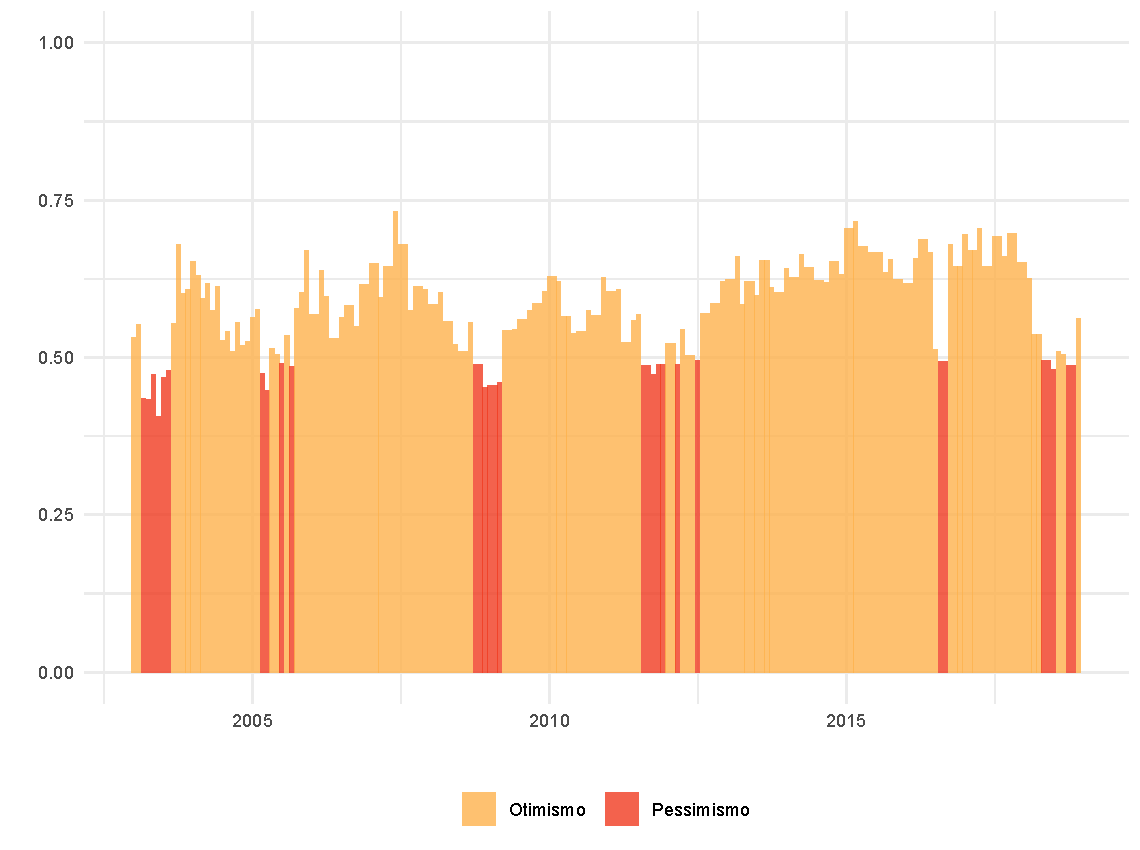
\includegraphics[width=\textwidth]{capitulos/figures/graf_indice_ggplot.pdf}
    \fonte{Elaboração própria}
    \label{fig:grafind}
\end{figure}


A Figura \ref{fig:grafind} apresenta a variação do índice proposto. Na barra abaixo da série é apresentado momentos de ``otimismo'' e ``pessimismo'' de acordo com o \textit{score}. De forma geral, percebe-se que o índice se mantem na maior parte do tempo de forma positiva - mesmo em momentos de crise. Argumenta-se que a abordagem do COPOM aos momentos críticos na conjuntura brasileira é dado de forma otimista. 

O índice de otimismo proposto pode ser utilizado como uma ferramenta de apoio à analise conjuntural brasileira, de tal forma que seria possível determinar a expressão do BCB para o período atual. Assim, este poderia servir como um indicador - \textit{proxy} - para o tipo de atuação do BCB frente a uma possível situação conjuntural mais crítica. 

\section{Exemplo de Aplicação}

Como proposto em \citeonline{shapiro2018measuring} e \citeonline{shapiro2019taking}, a partir de um índice de \textit{positividade} ou \textit{negatividade} é possível tentarmos entender o que aconteceria com a economia ou com esse índice, dados choques de algumas variáveis macroeconômicas.

Para entendermos o que poderia acontecer em alguns cenários, iremos nos basear em \citeonline{shapiro2019taking} e iremos reproduzir o exercício de função impulso resposta para algumas variáveis macroeconômicas brasileiras. Isso é, assumindo endogeneidade nas variáveis, estima-se um VAR para melhor compreender o que aconteceria se, por exemplo, num cenário de choque positivo no índice, como o Índice de Preços ao Consumidor Amplo (IPCA) acumulado em 12 meses reagiria. 

\subsection{Base de Dados e Período de Estimação}

Para a realização deste exercício, utilizaremos o IPCA acumulado em 12 meses, como uma \textit{proxy} da inflação acumulada; e o Índice de Atividade Econômica do Banco Central (IBC-Br) - com ajuste sazonal. respectivamente, representam as séries de número 13522 e 24364, do SGS - Sistema Gerenciador de Séries Temporais (BCB). Além dessas séries, utilizaremos, também, o índice proposto em (\ref{indice}). 

Uma primeira questão que nos toma, é se as séries são estacionárias. Para nos certificarmos da presença ou não de estacionariedade, utilizaremos o teste de Dickey-Fuller aumentado (ADF). Esse teste tem como hipótese nula ($H_0$) a presença de raiz unitária; usualmente, sua hipótese alternativa ($H_A$) é aceita como presença de estacionariedade - condição necessária para a estimação do VAR.  

\begin{table}[!h]
\centering
\caption{Testes de raiz unitárias para as variáveis utilizadas no exercício}
\begin{tabular}{llllc}
  \hline
Variáveis & ADF (-) & ADF (c) & ADF (ct) & Integração \\ 
  \hline
IbcBr & 1.9531 & -2.1196 & -0.7971 & I(1)\\ 
IPCA*** & -2.7598 & -4.3018*** & -4.1054*** & I(0) \\ 
Índice & -0.4107 & -3.7810*** & -3.9939*** & I(0)\\ 
D(IbcBr) & -7.4123*** & -7.6612*** & -7.8751*** & I(0)\\ 
D(IPCA) & -6.4765*** & -6.5740*** & -6.6907*** & I(0)\\ 
D(Índice) & -11.4768*** & -11.4444*** & -11.4429*** & I(0)\\ 
Est. de Teste (Tau) (10\%) & -1.6200 & -2.5700 & -3.1300 & -\\ 
Est. de Teste (Tau) (5\%) & -1.9500 & -2.8800 & -3.4300 & -\\ 
Est. de Teste (Tau) (1\%) & -2.5800 & -3.4600 & -3.9900 & -\\ 
   \hline
\end{tabular} \label{adf}
\fonte{Elaboração própria.}
\nota{* Rejeita-se a hipótese nula a nível de 10\%, ** Rejeita-se a hipótese nula a nível de 5\%, *** Rejeita-se a hipótese nula a nível de 1\%}
\end{table}

A Tabela \ref{adf} apresenta os resultados dos testes de raiz unitária realizados. De acordo com os testes realizados, podemos rejeitar a hipótese de presença de raiz unitária para todas as séries em diferença. Trabalhando em nível, entretanto, só podemos rejeitar esta hipótese para as séries IPCA e índice - mesmo assim, para as últimas duas séries, somente com presença de intercepto e tendência.

É necessário, desta forma, trabalharmos com a série \texttt{D(IbcBr)} - a série em diferênça do Índice de Atividade Econômica do Banco Central.

\subsection{O Modelo Estimado}

A partir do pacote \textit{vars} pode-se estipular a ordem do VAR, dado critérios de informação de akaike, Hannan-Quinn, e Bayesian Information Criterion; respectivamente AIC, HQ, e BIC \cite{pfaff2008var}. Foi verificado que para todos os critérios de informação apontaram para um VAR de segunda ordem. Isso é: foi regredido nas três variáveis utilizadas (D(IbcBr), IPCA, e índice) até a segunda ordem de defasagem de cada uma, de tal forma que o sistema de cada apresente 6 regressores. A equação estimada do VAR(2) para o indice, ficaria, então:
\begin{align*}
    indice_t = \Gamma_1 indice_{t-1} + \Gamma_2 indice_{t-2} &+ \Gamma_3 IPCA_{t-1} + \Gamma_4 IPCA_{t-2}\quad+ \\
                                                           & + \Gamma_5 \Delta IbcBr_{t-1} + \Gamma_6 \Delta IbcBr_{t-6} + const + trend + \epsilon
\end{align*}

\noindent
feito isso, e realizadas das estimações, pode-se estimar a função resposta ao impulso.

\subsection{Impulso Resposta ao Índice}
Como apresentado em (\ref{respostaimpulso}) em \citeonline{shapiro2019taking} e em \citeonline{jorda2005estimation}, realizamos o procedimento de estimação do VAR(2) e obtivemos suas funções de resposta ao impulso do índice.

\begin{figure}[!h]
    \centering
    \caption{Resposta das variáveis utilizadas a um choque em \textit{índice}}
    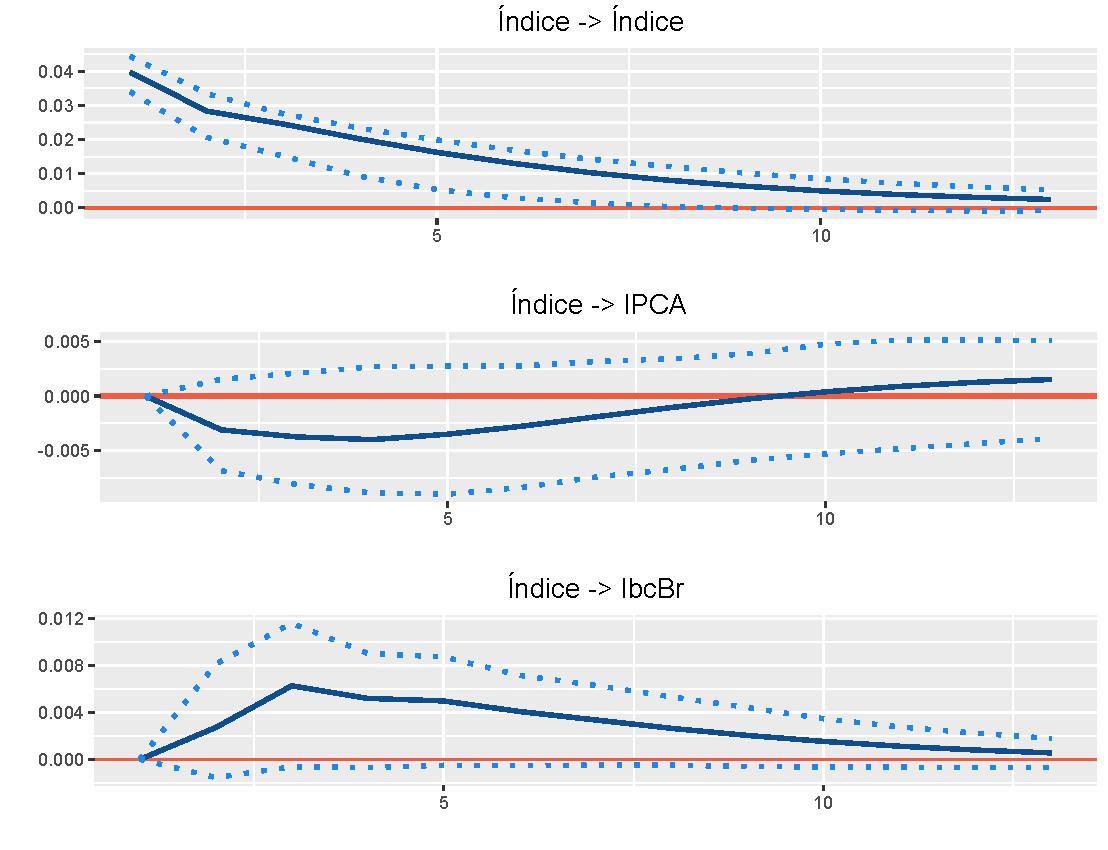
\includegraphics[width=.8\textwidth]{capitulos/figures/irf.pdf}
    \fonte{Elaboração própria}
    \label{fig:fri}
\end{figure}

A Figura \ref{fig:fri} apresenta a projeção para um choque em índice para um período posterior de 12 meses. Isto é, de acordo com a estimação, obtida a partir da \textit{identificação de cholesky} (ver \citeonline{enders2008applied}), dado um choque positivo no índice de otimismo obtido, a tendência de projeção seria que, para as variáveis obtidas:

\begin{enumerate}
    \item A varição do Índice de Atividade Econômica do Banco Central tenderia a ser positiva por um período de 12 meses a frente. Ainda, em cerca de 15 períodos esta voltaria ao seu estado original (não representado na figura);
    \item Em relação ao IPCA, o Índice de Preços ao Consumidor amplo sofreria uma queda inicial, em relação ao acumulado em 12 meses. Posteriormente, essa queda seria convertida em acréscimo, entretanto, com valor inferior a queda inicial. Após cerca de 17 períodos o valor do IPCA acumulado em 12 meses tenderia ao seu estado inicial (não representado na figura). 
\end{enumerate}

É válido salientar que há uma vasta opção de variáveis macroeconômicas brasileiras que poderiam ser utilizadas como referência para uma possível correlação com o índice de otimismo. Utilizamos o IPCA e o Ibc-Br como forma de aproximar o exercício da proposta inicial de \citeonline{shapiro2019taking}, visto que foram variáveis de escolhas próximas. Nada impede, entretanto, de utilizarmos outras variáveis como componentes do VAR - bem como nada impede a utilização de outras técnicas de estimação, ou mesmo testes para verificação de causalidade, por exemplo.





